\begin{titlepage}
    \ifdraft\BgThispage\fi
    \begin{center}
        % \fontfamily{phv}\selectfont
        % \AddToHook{shipout/background}{%
        %     \put (0in,-\paperheight){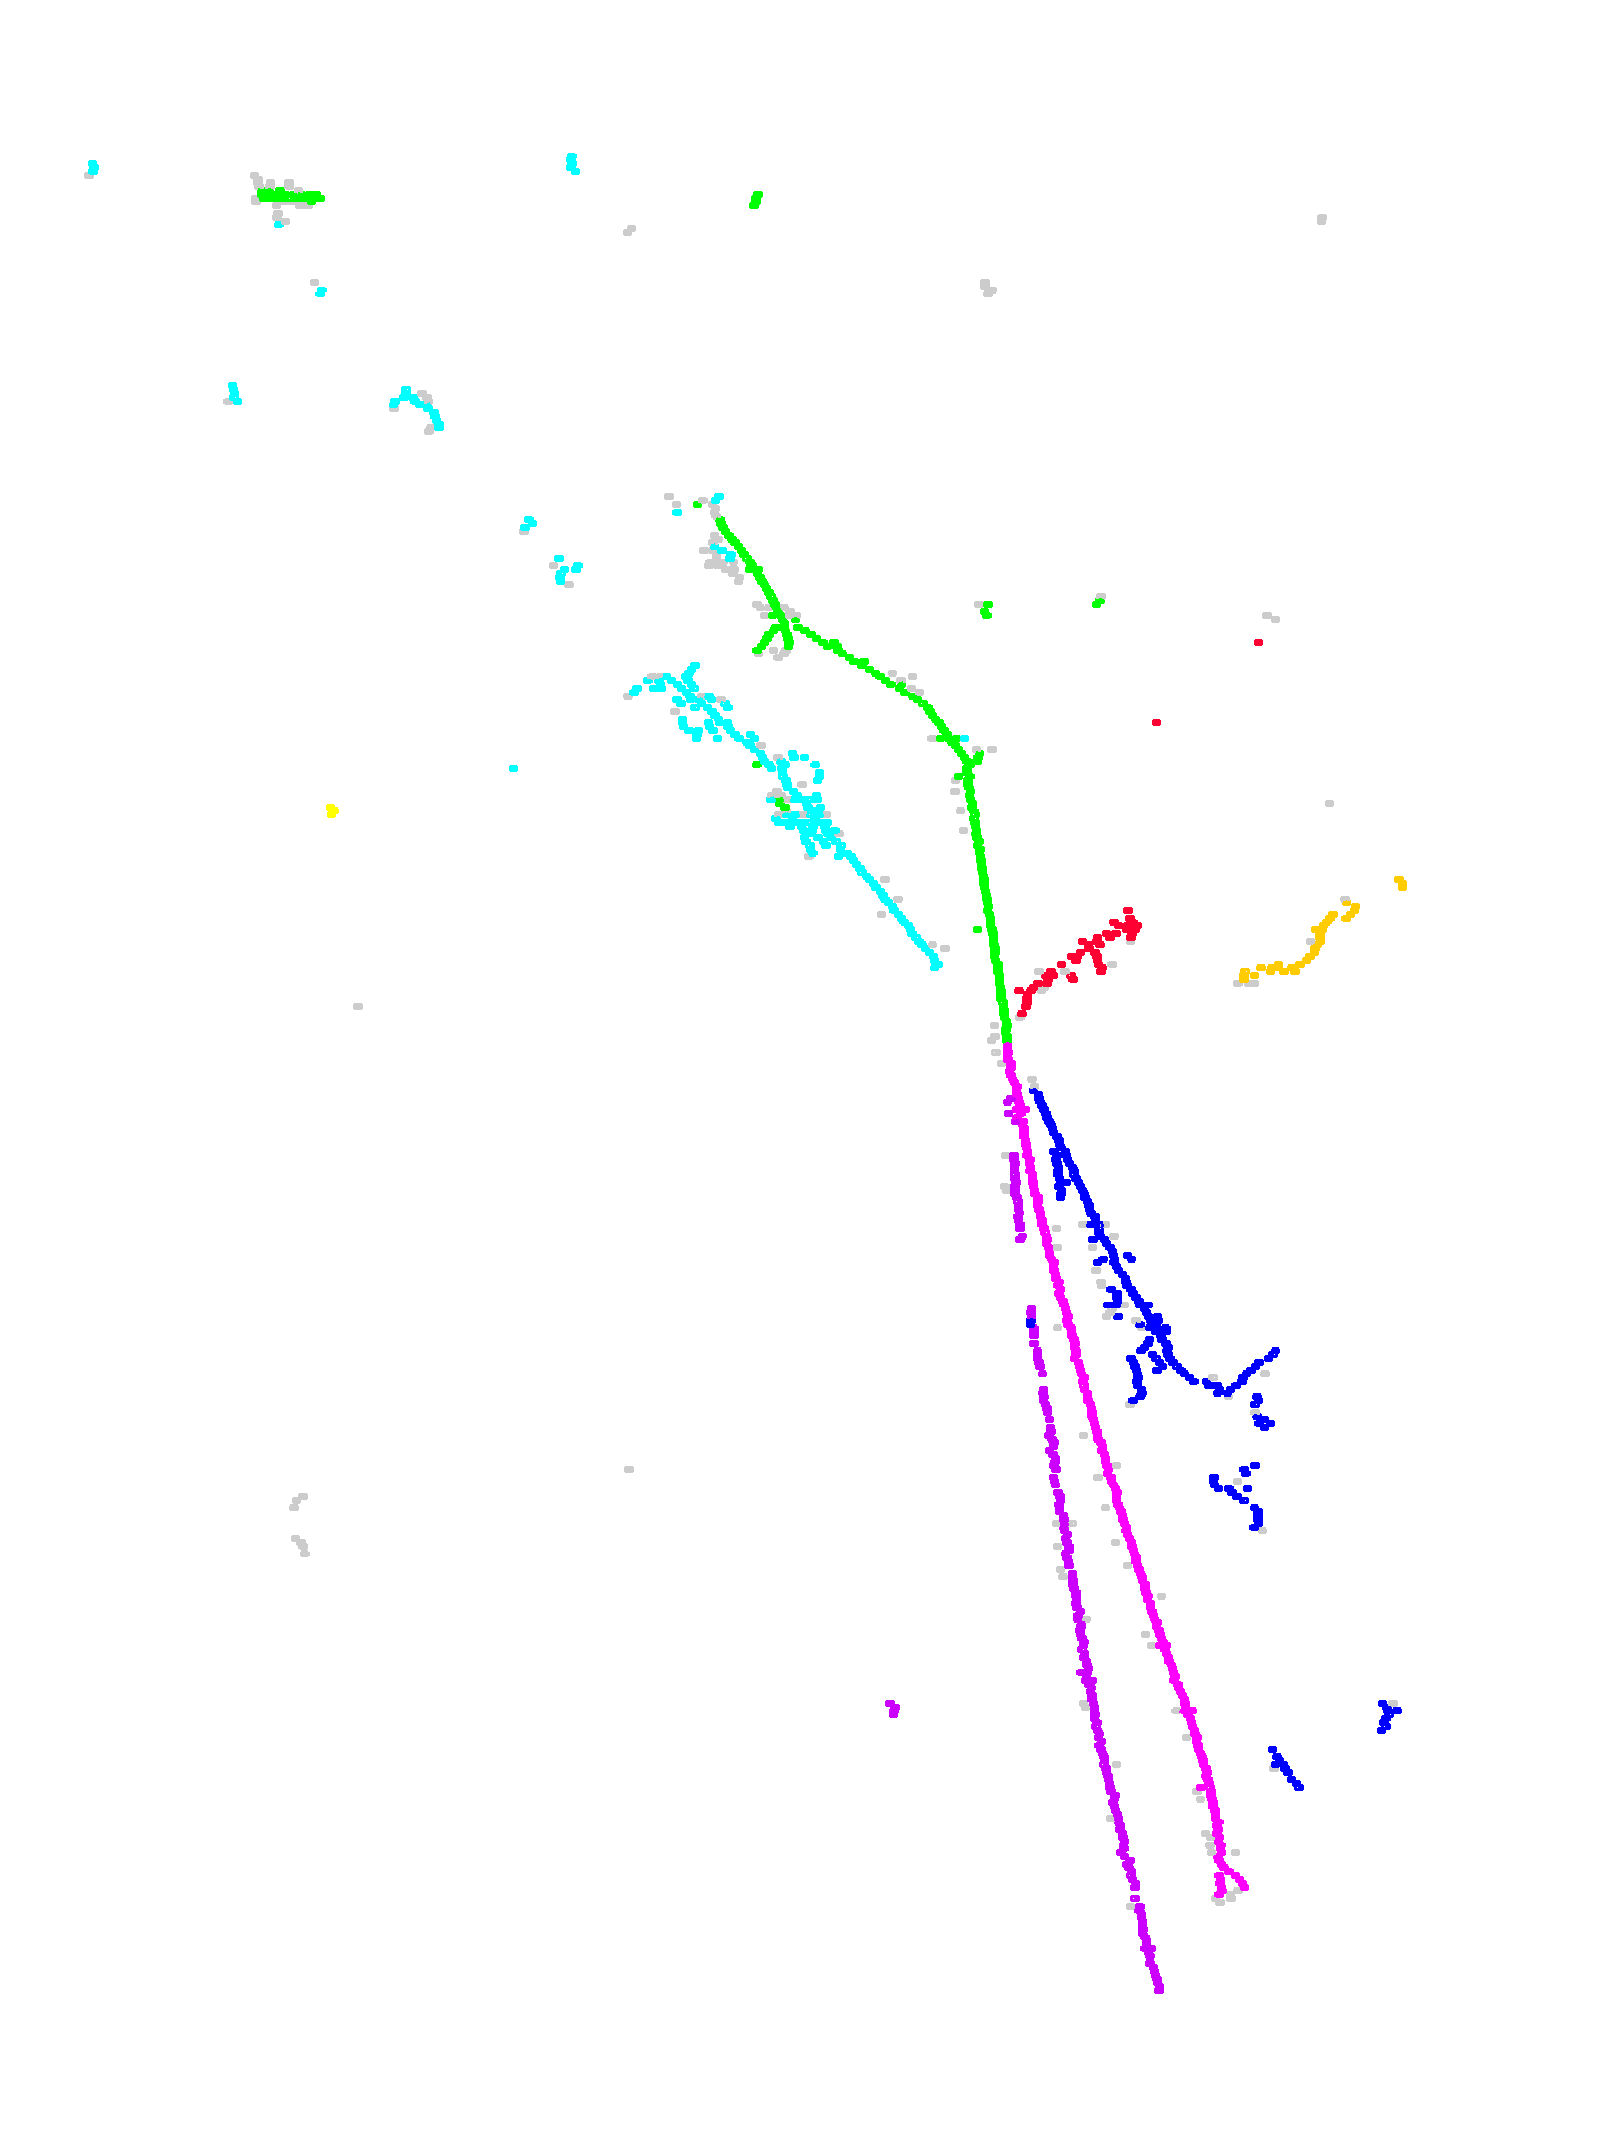
\includegraphics[width=\paperwidth,height=\paperheight]{6_figures/COVER/cover.pdf}}%
        % }

        {{Università degli Studi di Genova}}\par

        {Scuola di Scienze Matematiche, Fisiche e Naturali} \par

        \vspace{0.5cm}

        {Anno Accademico 2024/2025}

        \vfill

        Tesi di Laurea Magistrale in Fisica\par
        Curriculum di Fisica delle Interazioni Fondamentali

        \vfill

        \begin{minipage}{0.775\linewidth}
            \centering
            \huge
            \bfseries
            {\LARGE Opening Pandora's box}\par%
            {\Large A dedicated study of the automatic event reconstruction in the ICARUS-T600 experiment}%
        \end{minipage}

        \vfill

        \textbf{\small Candidato}\\{Mattia Sotgia}%
%
        \vfill%

        \begin{minipage}{0.45\linewidth}%
            \textbf{\small Relatrice}\par%
            {Dr. Alice Campani}\par\vspace{1em}%
            % {Universit\`a degli studi di Genova}\par\vspace{1em}
            \textbf{\small Relatore}\par%
            {Prof. Marco Pallavicini}%
            % \par{Universit\`a degli studi di Genova}
        \end{minipage}%
        \hfill%
        \begin{minipage}{0.45\linewidth}
            \raggedleft
            \textbf{\small Correlatrice}\par
            {Carla Biggio}
        \end{minipage}

        \vspace{2cm}

		Genova, 15 settembre 2025
        % Genova, 25 ottobre 2025
    \end{center}
\end{titlepage}
